% =====================================================================
% Capitolo 1 - Homework 1: cinematica diretta del braccio sinistro di Reachy 2
% (titolo impostato in main.tex con \capitolo{...}{capitolo1})
% Tabella della validazione generata da Homework1/risultati_test_pose.csv (test_pose.m).
% =====================================================================

\section{Scelta delle terne DH}
\label{sec:hw1-terne}

Le terne seguono la convenzione di Denavit-Hartenberg (Figura~\ref{fig:hw1-terne}).

\begin{itemize}
    \item Le $z_{i-1}$ sono poste lungo gli assi $i$ dei giunti, con verso dato dalla rotazione del giunto corrispondente.
    \item Le origini delle terne sono posizionate quindi come segue: $O_0 \equiv O_1 \equiv O_2$ nella spalla, $O_3$ nel gomito, $O_4 \equiv O_5 \equiv O_6$ nel polso, $O_7$ a met\`a delle dita della pinza.
    \item Le $x_i$ associate alle $z_i$ sono quasi tutte libere a causa dell'orientamento degli assi dei giunti, per cui sono state posizionate per essere coerenti con la posa iniziale $q$; l'unica eccezione è costituita da $x_4$, la cui direzione è fissata dalla normale comune tra $z_3$ e $z_4$, che è unica, e il cui verso lo impone la convenzione dal giunto $i$ al giunto $i+1$.
\end{itemize}

\noindent
In particolare $x_4$ \`e diretto dal gomito al polso, quindi $a_4 = +0.28$~m.
Gli assi $z_2$ e $z_6$ risultano invece diretti verso la spalla, mentre gomito e pinza stanno nel verso opposto: per questo $d_3 = -0.28$~m e $d_7 = -0.11$~m. I parametri sono riportati in Tabella~\ref{tab:hw1-dh}.

\begin{figure}[H]
\centering
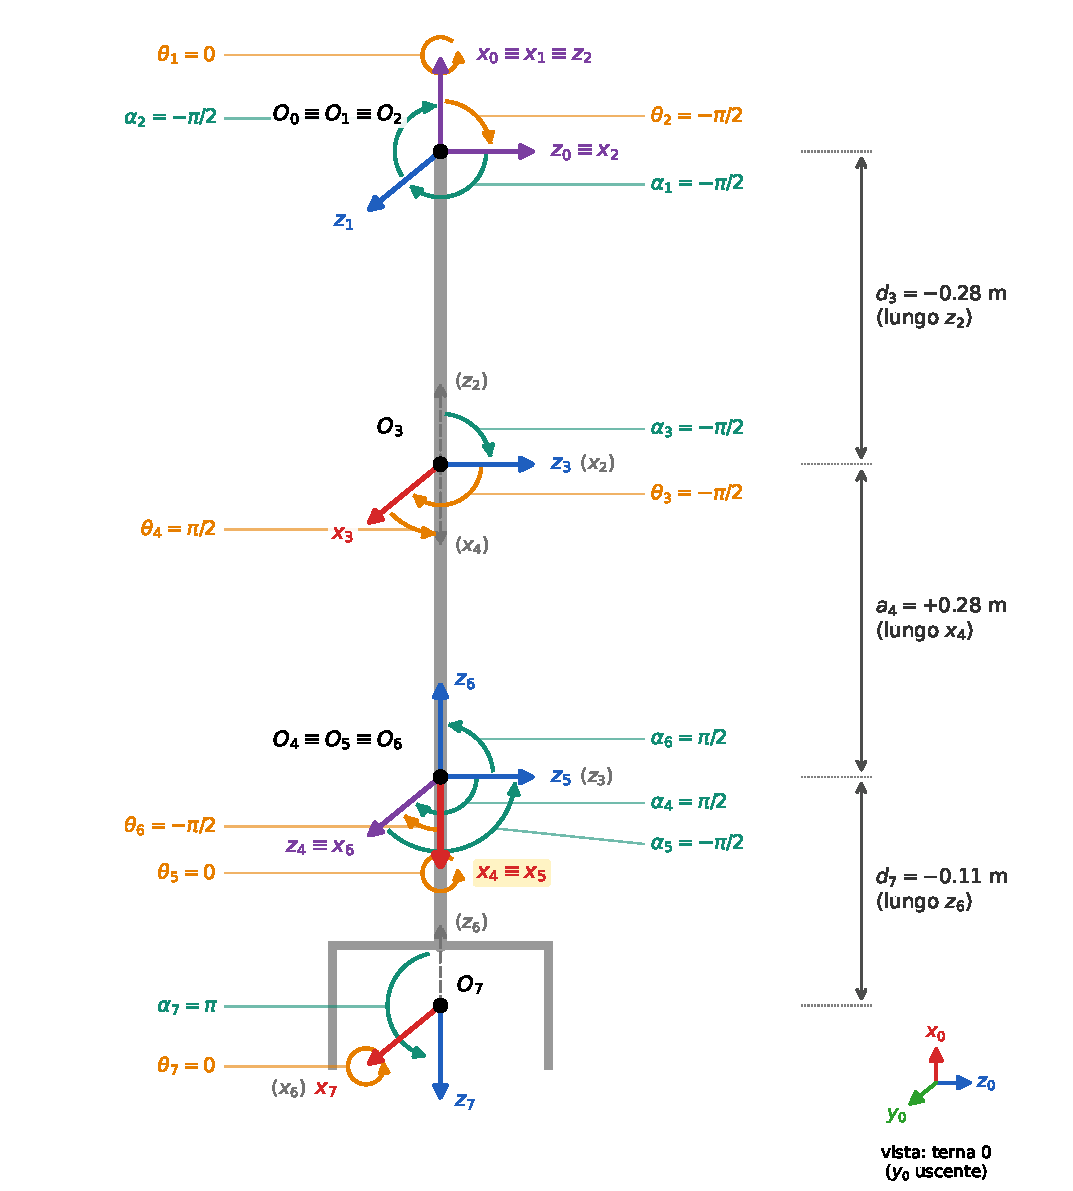
\includegraphics[width=0.85\textwidth]{images/terne_dh_convenzione.pdf}
\caption[Terne DH adottate nella posa di riferimento]{Terne DH adottate, nella posa di riferimento. Assi $x$ in rosso, assi $z$ in blu, assi coincidenti $x \equiv z$ in viola; $\theta_i$ in arancio, $\alpha_i$ in verde. Gli assi tratteggiati appartengono a un'altra terna. Distanze non in scala.}
\label{fig:hw1-terne}
\end{figure}

\begin{table}[H]
\centering
\begin{tabular}{|c|c|c|c|c|}
\hline
Link & $a_i$ (m) & $d_i$ (m) & $\theta_i$ & $\alpha_i$ \\
\hline
1 & $0$ & $0$ & $\theta_1$ & $-\pi/2$ \\
2 & $0$ & $0$ & $\theta_2$ & $-\pi/2$ \\
3 & $0$ & $-0.28$ & $\theta_3$ & $-\pi/2$ \\
4 & $0.28$ & $0$ & $\theta_4$ & $\pi/2$ \\
5 & $0$ & $0$ & $\theta_5$ & $-\pi/2$ \\
6 & $0$ & $0$ & $\theta_6$ & $\pi/2$ \\
7 & $0$ & $-0.11$ & $\theta_7$ & $\pi$ \\
\hline
\end{tabular}
\caption{Parametri DH adottati.}
\label{tab:hw1-dh}
\end{table}

\section{\texorpdfstring{Confronto con le terne implicite nel testo}{Confronto con le terne implicite nel testo}}
\label{sec:hw1-confronto}

Con le terne di Figura~\ref{fig:hw1-terne}, la posa di riferimento del testo non si ottiene con il vettore assegnato $q = [0,\ -\pi/2,\ -\pi/2,\ -\pi/2,\ 0,\ \pi/2,\ 0]$.
Quel vettore, insieme all'offset di \texttt{moveLeftArm} e ai limiti articolari forniti, corrisponde infatti a una diversa scelta di $x_4$.
Con $\theta_4 = -\pi/2$, ruotando $x_3$ attorno a $z_3$, l'asse $x_4$ risulta diretto dal polso verso la spalla (Figura~\ref{fig:hw1-terne-testo}).

\noindent
Con questa rappresentazione cambiano solo le righe 4 e 5 della tabella: $a_4 = -0.28$~m, $\alpha_4 = -\pi/2$ e $\alpha_5 = \pi/2$, necessari per mantenere $z_4$ concorde con la rotazione del giunto 5 (Tabella~\ref{tab:hw1-dh-testo}).
Le due tabelle descrivono lo stesso braccio e differiscono solo per le variabili di giunto:
\[
\theta_{\text{adottate}} = q_{\text{testo}} + [0,\ 0,\ 0,\ \pi,\ 0,\ -\pi,\ 0].
\]
Anche $\theta_6$ cambia di $\pi$ perch\'e, per $\theta_5 = 0$, $x_5$ coincide con $x_4$ e si ribalta con esso.

\begin{figure}[H]
\centering
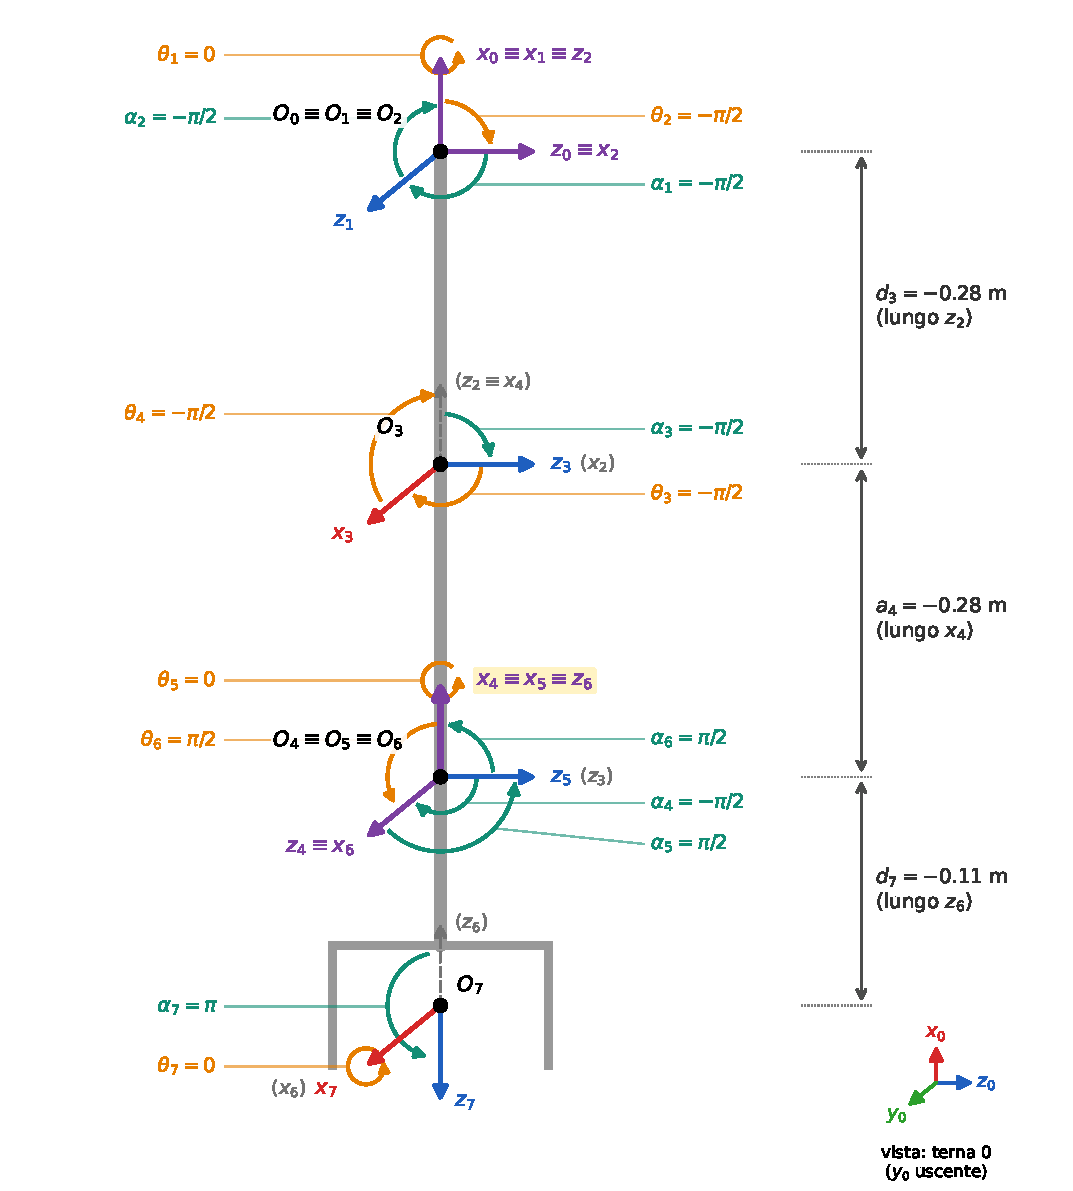
\includegraphics[width=0.85\textwidth]{images/terne_dh_adottata.pdf}
\caption[Terne DH implicite nei dati del testo]{Terne DH implicite nei dati del testo, con $x_4$ diretto verso la spalla. Rispetto alla Figura~\ref{fig:hw1-terne} cambiano solo le terne 4 e 5 e gli angoli $\theta_4$, $\alpha_4$, $\alpha_5$, $\theta_6$.}
\label{fig:hw1-terne-testo}
\end{figure}

\begin{table}[H]
\centering
\begin{tabular}{|c|c|c|c|c|}
\hline
Link & $a_i$ (m) & $d_i$ (m) & $\theta_i$ & $\alpha_i$ \\
\hline
4 & $-0.28$ & $0$ & $\theta_4$ & $-\pi/2$ \\
5 & $0$ & $0$ & $\theta_5$ & $\pi/2$ \\
\hline
\end{tabular}
\caption{Righe 4 e 5 della tabella DH con le terne implicite nel testo; le altre righe coincidono con la Tabella~\ref{tab:hw1-dh}.}
\label{tab:hw1-dh-testo}
\end{table}

Per usare la tabella adottata sono stati quindi aggiornati, per i giunti 4 e 6, la posa di riferimento, l'offset in \texttt{moveLeftArm} e i limiti articolari in \texttt{direct\_kin} (Tabella~\ref{tab:hw1-dati}).
Il valore inviato al simulatore, $q + \text{offset}$, resta lo stesso, e la posa di riferimento corrisponde ancora allo zero di CoppeliaSim.

\begin{table}[H]
\centering
\renewcommand{\arraystretch}{1.2}
\begin{tabular}{|c|l|c|c|}
\hline
Giunto & Dato (rad) & Testo & Adottato \\
\hline
4 & Posa di riferimento & $-\pi/2$ & $\pi/2$ \\
4 & Offset per CoppeliaSim & $\pi/2$ & $-\pi/2$ \\
4 & Limiti & $[-3.8208,\ -1.4708]$ & $[-0.6792,\ 1.6708]$ \\
\hline
6 & Posa di riferimento & $\pi/2$ & $-\pi/2$ \\
6 & Offset per CoppeliaSim & $-\pi/2$ & $\pi/2$ \\
6 & Limiti & $[1.2208,\ 1.9208]$ & $[-1.9208,\ -1.2208]$ \\
\hline
\end{tabular}
\caption{Dati dei giunti 4 e 6: valori del testo e valori adottati.}
\label{tab:hw1-dati}
\end{table}

La posa di riferimento adottata \`e quindi
\[
q = \left[0,\ -\tfrac{\pi}{2},\ -\tfrac{\pi}{2},\ \tfrac{\pi}{2},\ 0,\ -\tfrac{\pi}{2},\ 0\right].
\]

\section{Cinematica diretta}
\label{sec:hw1-cinematica}

La matrice $A_e^b(q) = A_0^b\, A_1^0(q_1) \cdots A_7^6(q_7)$ \`e calcolata una sola volta in forma simbolica da \texttt{calcola\_trasform\_mat.m} e salvata in \texttt{matrici\_robot.mat}.
La funzione
\begin{lstlisting}[language=Matlab]
[p, phi, R, quat] = direct_kin(q, 'ZYZ');   % oppure 'RPY'
\end{lstlisting}
sostituisce i valori dei giunti e restituisce la posizione $p$, gli angoli di Eulero richiesti, la matrice di rotazione $R$ e il quaternione $[\eta;\ \epsilon]$.
I giunti fuori dai limiti articolari vengono saturati con un warning; nei casi singolari ($\sin\vartheta = 0$ per ZYZ, $\cos\vartheta = 0$ per RPY) si pone $\varphi = 0$.

\section{Validazione}
\label{sec:hw1-validazione}

La funzione \texttt{test\_pose.m} invia al simulatore 20 configurazioni con \texttt{moveLeftArm} e confronta la posizione $p$ calcolata da \texttt{direct\_kin} con la posizione $p_c$ della terna \texttt{l\_EE\_FRAME} letta da CoppeliaSim.
Le configurazioni sono la posa di riferimento (test 1), un giunto alla volta al 15\% e all'85\% del suo intervallo (test 2--15) e cinque configurazioni casuali entro i limiti (test 16--20).

\begin{table}[H]
\centering
\footnotesize
\setlength{\tabcolsep}{3pt}
\renewcommand{\arraystretch}{1.15}
\begin{tabular}{|c|ccccccc|ccc|c|}
\hline
 & \multicolumn{7}{c|}{$q$ (rad)} & \multicolumn{3}{c|}{$p_c$ (m)} & $\lVert p - p_c \rVert$ \\
Test & $q_1$ & $q_2$ & $q_3$ & $q_4$ & $q_5$ & $q_6$ & $q_7$ & $x$ & $y$ & $z$ & (mm) \\
\hline
1 & $0$ & $-\pi/2$ & $-\pi/2$ & $\pi/2$ & $0$ & $-\pi/2$ & $0$ & $0.046$ & $0.371$ & $0.349$ & $0.05$ \\
2 & $-2.20$ & $-\pi/2$ & $-\pi/2$ & $\pi/2$ & $0$ & $-\pi/2$ & $0$ & $0.532$ & $0.005$ & $1.378$ & $1.37$ \\
3 & $2.20$ & $-\pi/2$ & $-\pi/2$ & $\pi/2$ & $0$ & $-\pi/2$ & $0$ & $-0.537$ & $0.194$ & $1.378$ & $1.39$ \\
4 & $0$ & $-1.10$ & $-\pi/2$ & $\pi/2$ & $0$ & $-\pi/2$ & $0$ & $0.093$ & $0.642$ & $0.498$ & $0.37$ \\
5 & $0$ & $1.10$ & $-\pi/2$ & $\pi/2$ & $0$ & $-\pi/2$ & $0$ & $0.040$ & $0.338$ & $1.653$ & $1.55$ \\
6 & $0$ & $-\pi/2$ & $-3.77$ & $\pi/2$ & $0$ & $-\pi/2$ & $0$ & $0.046$ & $0.371$ & $0.349$ & $0.32$ \\
7 & $0$ & $-\pi/2$ & $0.63$ & $\pi/2$ & $0$ & $-\pi/2$ & $0$ & $0.046$ & $0.371$ & $0.349$ & $0.33$ \\
8 & $0$ & $-\pi/2$ & $-\pi/2$ & $-0.33$ & $0$ & $-\pi/2$ & $0$ & $0.387$ & $0.175$ & $0.847$ & $1.24$ \\
9 & $0$ & $-\pi/2$ & $-\pi/2$ & $1.32$ & $0$ & $-\pi/2$ & $0$ & $0.141$ & $0.351$ & $0.361$ & $0.21$ \\
10 & $0$ & $-\pi/2$ & $-\pi/2$ & $\pi/2$ & $-0.24$ & $-\pi/2$ & $0$ & $0.041$ & $0.344$ & $0.345$ & $0.18$ \\
11 & $0$ & $-\pi/2$ & $-\pi/2$ & $\pi/2$ & $0.24$ & $-\pi/2$ & $0$ & $0.050$ & $0.396$ & $0.359$ & $0.21$ \\
12 & $0$ & $-\pi/2$ & $-\pi/2$ & $\pi/2$ & $0$ & $-1.82$ & $0$ & $0.072$ & $0.365$ & $0.352$ & $0.21$ \\
13 & $0$ & $-\pi/2$ & $-\pi/2$ & $\pi/2$ & $0$ & $-1.33$ & $0$ & $0.019$ & $0.375$ & $0.352$ & $0.18$ \\
14 & $0$ & $-\pi/2$ & $-\pi/2$ & $\pi/2$ & $0$ & $-\pi/2$ & $-1.10$ & $0.045$ & $0.371$ & $0.349$ & $0.19$ \\
15 & $0$ & $-\pi/2$ & $-\pi/2$ & $\pi/2$ & $0$ & $-\pi/2$ & $1.10$ & $0.046$ & $0.371$ & $0.349$ & $0.21$ \\
16 & $-0.42$ & $0.55$ & $-4.08$ & $0.12$ & $-0.20$ & $-1.80$ & $-0.79$ & $-0.201$ & $0.638$ & $0.948$ & $0.77$ \\
17 & $-0.78$ & $-0.26$ & $-1.38$ & $0.34$ & $0.10$ & $-1.74$ & $0.95$ & $0.341$ & $0.474$ & $1.332$ & $1.50$ \\
18 & $-2.38$ & $0.43$ & $-1.99$ & $0.61$ & $-0.20$ & $-1.74$ & $0.76$ & $-0.157$ & $0.684$ & $1.279$ & $1.57$ \\
19 & $2.35$ & $-0.47$ & $-0.60$ & $1.20$ & $0.22$ & $-1.80$ & $-1.16$ & $-0.040$ & $0.811$ & $1.215$ & $1.23$ \\
20 & $-1.66$ & $0.95$ & $-3.59$ & $0.35$ & $0.26$ & $-1.55$ & $0.48$ & $-0.016$ & $0.750$ & $0.991$ & $1.05$ \\
\hline
\end{tabular}
\caption{Configurazioni di test, posizione dell'end-effector in CoppeliaSim ed errore del modello.}
\label{tab:hw1-validazione}
\end{table}

\noindent
L'errore medio \`e 0.71~mm e il massimo 1.57~mm, circa lo 0.2\% della lunghezza del braccio (0.67~m).
Il residuo \`e dovuto ai dati arrotondati, non alla tabella DH.
